\chapter{Benutzeranleitung}
Diese Benutzeranleitung dient der leichten Erlernbarkeit der Software. Für Benutzer ohne Kenntnisse des Lightweight M2M (LwM2M) Protokolls empfiehlt sich die Spezifikationen des Ressourcenmodells (http://openmobilealliance.org/wp/OMNA/LwM2M/LwM2MRegistry.html) als Nachschlagewerk. Für das Grundlegende Verständnis von LwM2M kann das Kapitel \ref{sec:lwm2m} konsultiert werden. Die Benutzeranleitung ist inhaltlich nach den implementierten Use Cases (siehe Kapitel \ref{sec:usecases}) aufgebaut.

Voraussetzung für die Nutzung ist eine erfolgreiche Installation des Smartmanagers (siehe Kapitel \ref{sec:installation}). 

\section{Benutzerlogin}
\begin{itemize}
\item Der Smartmanager kann unter folgender URL benutzt werden: https://server.url:8443/smartmanager/
\item Auf der Startseite erscheint ein Loginfenster. Bevor die Applikation benutzt werden kann, muss ein gültiges Login getätigt werden.
\end{itemize}

\begin{figure}[H]
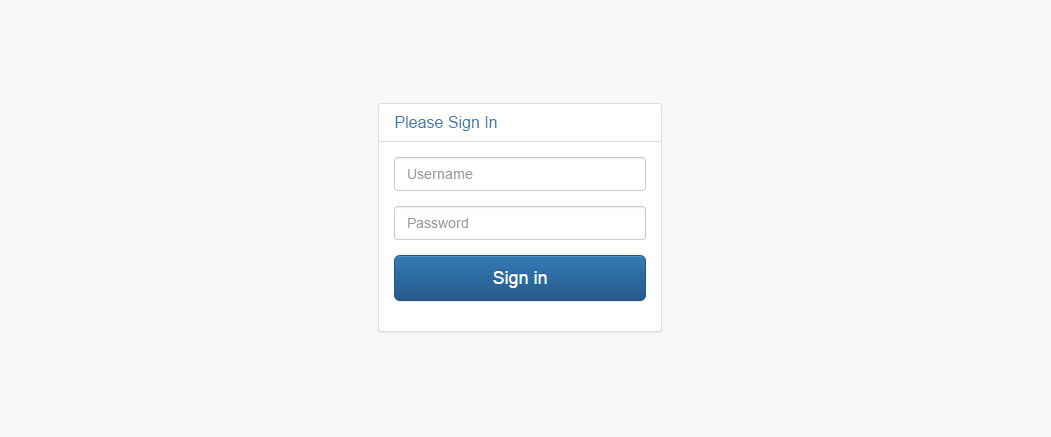
\includegraphics[scale=0.57]{../05_Schlussbericht/images/benutzeranleitung/login.png}
\end{figure}
\begin{itemize}
\item Sofern kein Login vorliegt, muss der Administrator konsultiert werden, welcher Benutzername und Passwort aushändigen kan
\item Das Standard-Login für den Administrator ist Username: admin, Password: admin
\end{itemize}
\newpage

\section{Benutzerverwaltung}
Die Benutzerverwaltung unterscheidet sich für Benutzer und den Administrator. Benutzer können zur Zeit lediglich ihr Kennwort zurücksetzen. Der Administrator kann sein eigenes Kennwort zurücksetzen, neue Benutzer anlegen und Benutzer löschen.

Die Benutzerverwaltung kann mit einem Klick auf den eigenen Benutzernamen am oberen rechten Bildschirmrand geöffnet werden.
\begin{figure}[H]
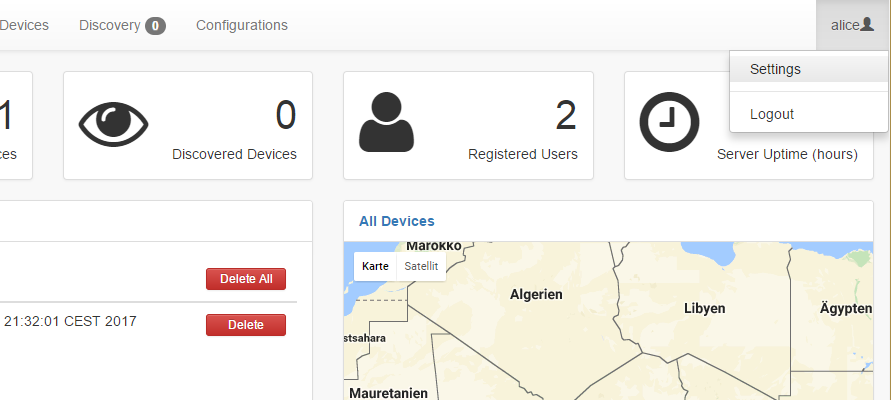
\includegraphics[scale=0.65]{../05_Schlussbericht/images/benutzeranleitung/usersettings.png}
\end{figure}

\subsubsection{Eigenes Kennwort ändern}
\begin{itemize}
\item Mit einem Klick auf ''Change password'' öffnet sich ein neues Fenster
\item Das bestehende Kennwort muss einmal- und das neue Kennwort zweimal eingegeben werden
\end{itemize}

\begin{figure}[H]
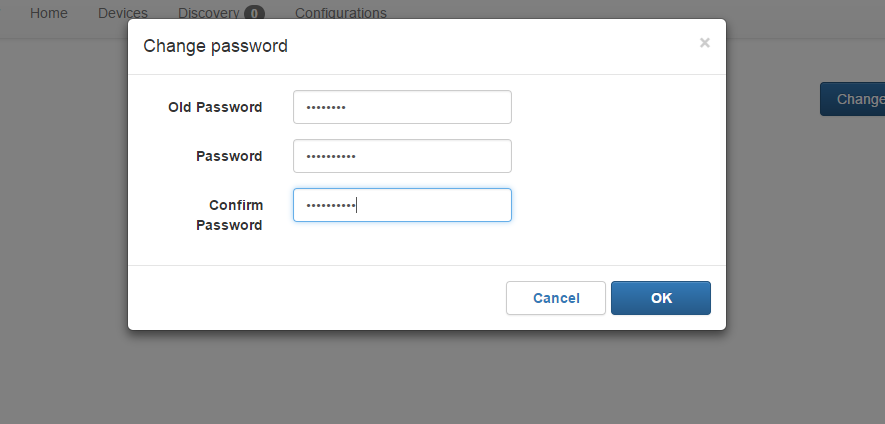
\includegraphics[scale=0.65]{../05_Schlussbericht/images/benutzeranleitung/change_password.png}
\end{figure}
\newpage

\subsubsection{Neuen Benutzer erstellen}
Neue Benutzer können nur als Administrator erstellt werden. Sobald man ''Create new User'' klickt, öffnet sich ein neues Fenster.

\begin{figure}[H]
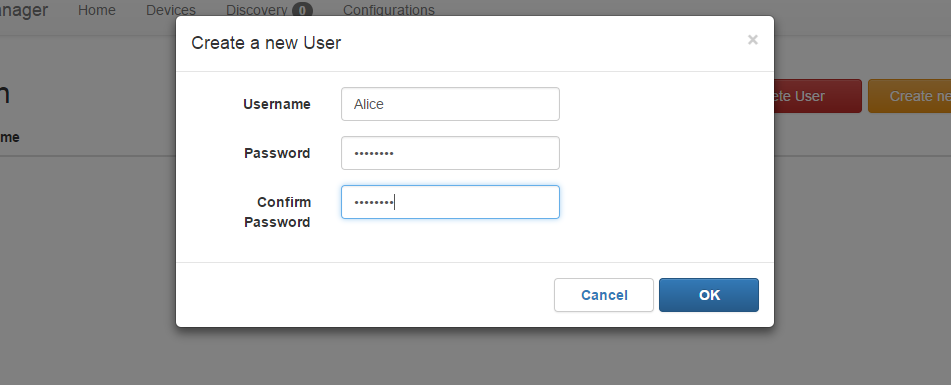
\includegraphics[scale=0.6]{../05_Schlussbericht/images/benutzeranleitung/create_new_user.png}
\end{figure}
Der Benutzername muss dabei aus mindestens 4 Zeichen bestehen.

\subsubsection{Benutzer löschen}
Benutzer können unter ''Delete User'' gelöscht werden. Im Drop-Down Menü kann der entsprechende Benutzer gelöscht werden. Es ist nicht möglich, den Admin zu löschen.
\begin{figure}[H]
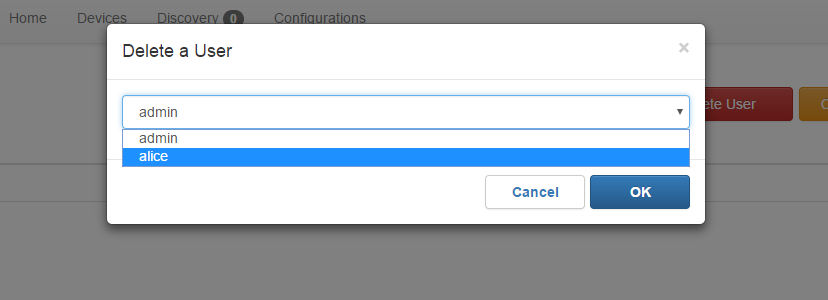
\includegraphics[scale=0.7]{../05_Schlussbericht/images/benutzeranleitung/delete_user.png}
\end{figure}
\newpage

\section{Gruppenverwaltung}
Auf der ''Devices''-Seite können Gruppen verwaltet werden. Auf der linken Seite befindet sich der Navigationsbaum. 

\begin{figure}[H]
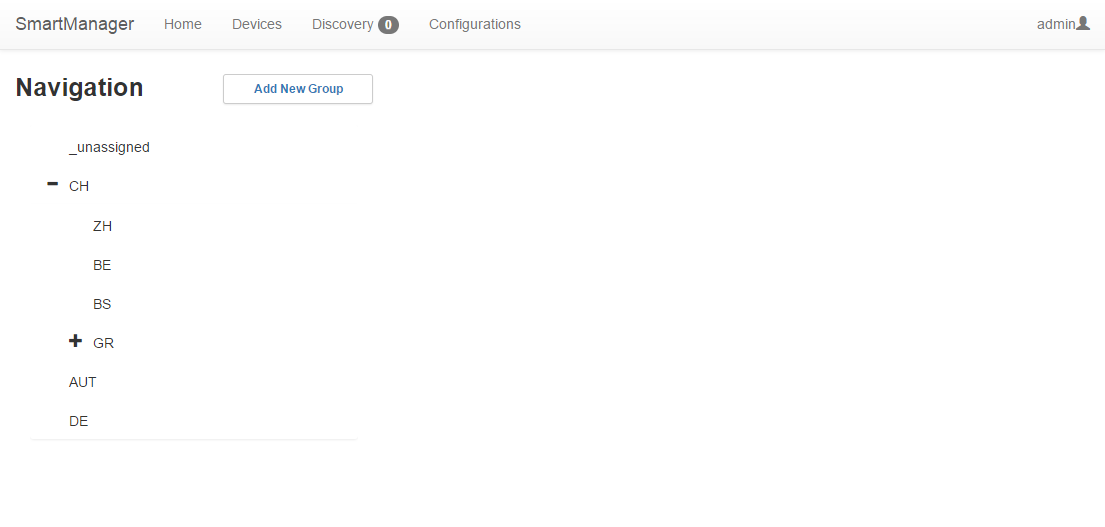
\includegraphics[scale=0.57]{../05_Schlussbericht/images/benutzeranleitung/gruppen_navigation.png}
\end{figure}

Mit einem Klick auf ''Add New Group'' wird eine neue Gruppe auf höchster Ebene angelegt. Einzig der Name der neuen Gruppe muss einzigartig sein, ansonsten existieren keine Einschränkungen. Sobald man in der Navigation eine Gruppe anklickt, erscheint die Gruppenansicht im Hauptfenster.

\begin{figure}[H]
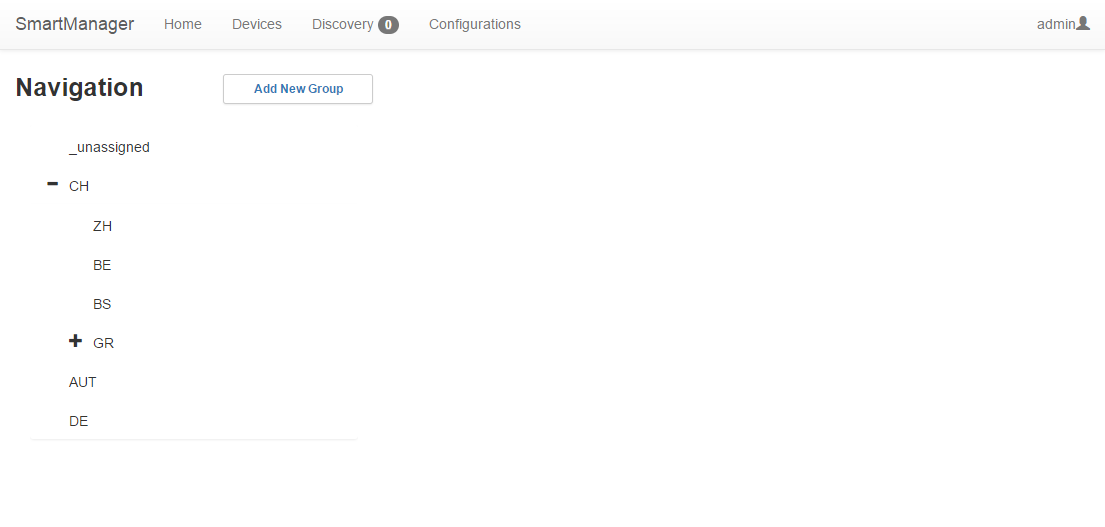
\includegraphics[scale=0.57]{../05_Schlussbericht/images/benutzeranleitung/gruppen_navigation.png}
\end{figure}

\subsubsection{Neue Kindsgruppe hinzufügen}
Unter ''Add New Child Group'' kann der Gruppe eine neue Kindsgruppe hinzugefügt werden. Einzig der Name darf nicht mehrfach vorkommen, ansonsten existieren keine Einschränkungen.

\subsubsection{Gruppenmitglieder verwalten}
Unter ''Group Members'' können die direkten Kindskomponenten (Devices und Gruppen) hinzugefügt- oder entfernt werden.

\begin{figure}[H]
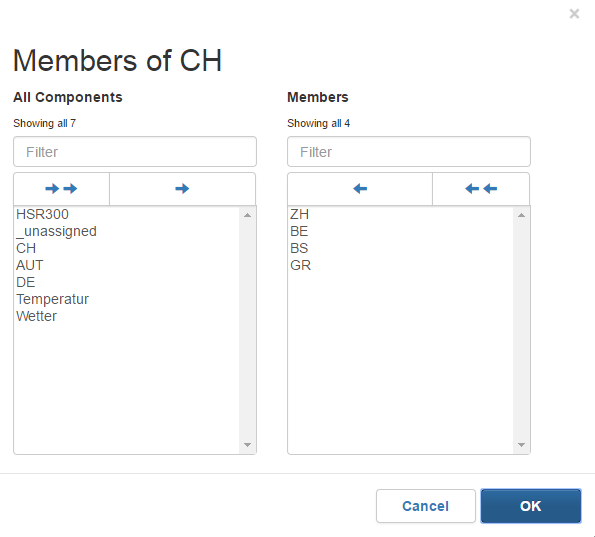
\includegraphics[scale=0.65]{../05_Schlussbericht/images/benutzeranleitung/gruppenmitglieder.png}
\end{figure}

Auf der linken Seite sind sämtliche Komponenten enthalten, welche noch nicht Mitglieder der Gruppe sind, auf der rechten Seite sind alle Mitglieder. Bei zuvielen Einträgen kann unter ''Filter'' nach dem Namen gesucht werden. 

Folgende Regeln gelten für das Setzen von Gruppenmitgliedern:
\begin{itemize}
\item Devices können in mehreren Gruppen Mitglied sein
\item Gruppen können nur in einer Gruppe Mitglied sein
\item Wird eine Gruppe als Mitglied gesetzt, so wird sie bei einer anderen Gruppe als Mitglied entfernt
\item Ein direkter oder indirekter Vor- oder Nachfahre der Gruppe kann nicht als Mitglied hinzugefügt werden
\item die Gruppe ''\_unassigned'' kann nicht als Mitglied hinzugefügt werden
\end{itemize}

\subsubsection{Gruppenmitgliedschaften verwalten}
Unter ''Group Memberships'' kann die direkte Elterngruppe hinzugefügt- oder entfernt werden.

Folgende Regeln gelten für das Setzen von Gruppenmitgliedschaften:
\begin{itemize}
\item Eine Gruppe kann genau eine Elterngruppe haben
\item Die Gruppe ''\_unassigned'' kann nicht als Elterngruppe gesetzt werden
\item Direkte- oder indirekte Nachfahren können nicht als Elterngruppe gesetzt werden
\end{itemize}
\newpage

\section{Konfigurationen verwalten}
Auf der ''Configurations''-Seite kann man eigene Konfigurationen erstellen, bearbeiten und löschen.

\begin{figure}[H]
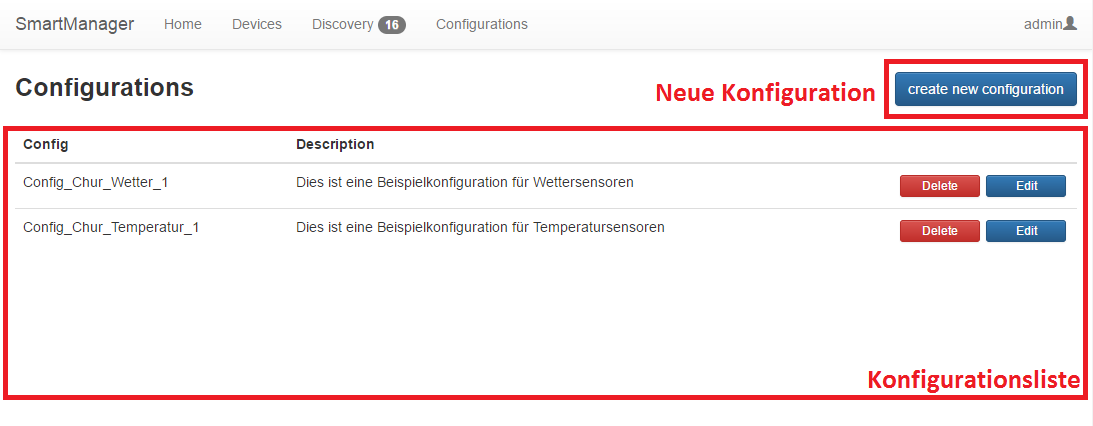
\includegraphics[scale=0.57]{../05_Schlussbericht/images/benutzeranleitung/configurations_overview.png}
\end{figure} 

\subsubsection{Konfiguration erstellen}
Unter ''create new configuration'' erstellt man eine neue Konfiguration.

\begin{figure}[H]
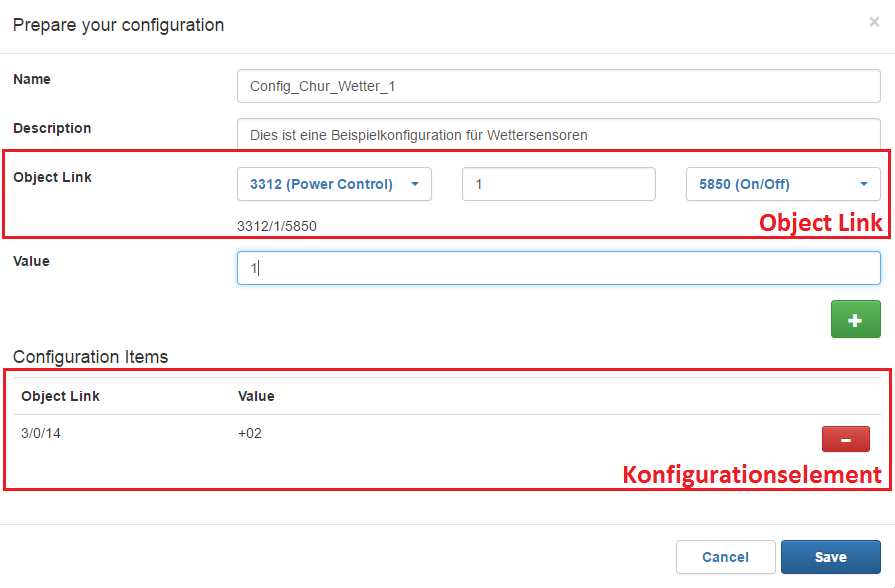
\includegraphics[scale=0.57]{../05_Schlussbericht/images/benutzeranleitung/create_configuration.png}
\end{figure} 

\begin{itemize}
\item Im Namensfeld kann ein beliebiger Name der Konfiguration eingegeben werden
\item Im Descriptionfeld kann eine beliebige Beschreibung eingegeben werden
\item Die Object Link Zeile wählt die zu beschreibende Ressource aus. Es werden dabei nur Ressourcen angezeigt, welche die Operation ''Write'' unterstützen
\item Im Value Feld wird der Wert für die Ressource eingetragen. Gegebenenfalls sollte die Spezifikation des Ressourcenmodells konsultiert werden
\item Unten sind die Konfigurationselemente tabellarisch ersichtlich
\end{itemize}

\section{Device Discovery}
Für das Discovery müssen sich Devices am Server registrieren. Auf der ''Discovery''-Seite sind registrierte- und noch nicht hinzugefügte Devices tabellarisch aufgelistet.

\begin{figure}[H]
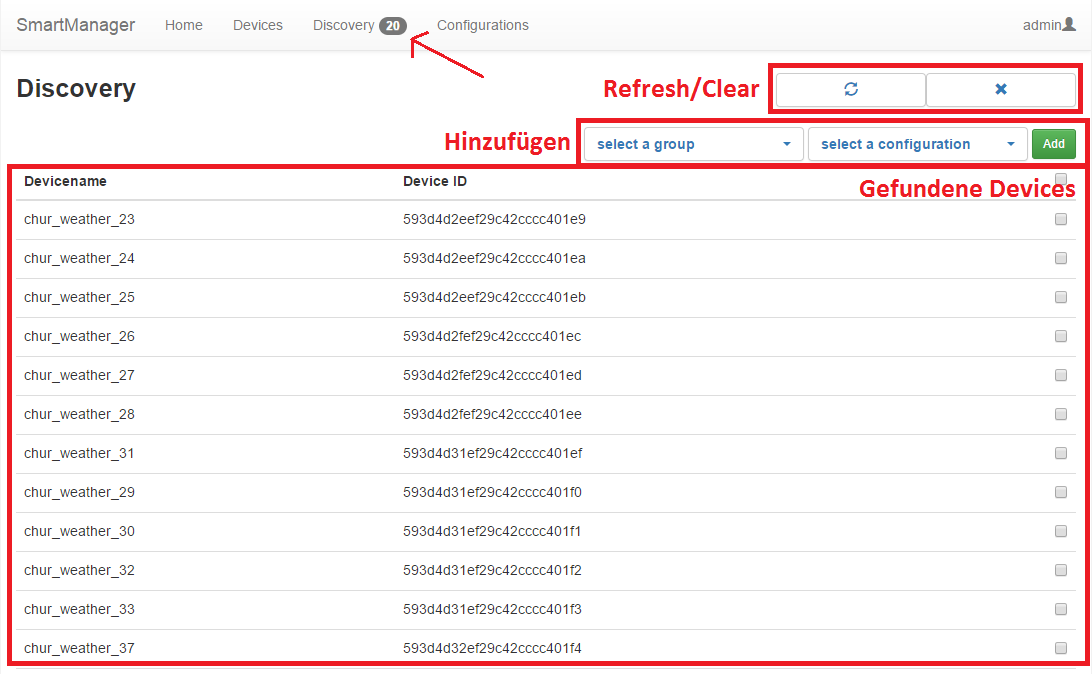
\includegraphics[scale=0.57]{../05_Schlussbericht/images/benutzeranleitung/discovery.png}
\end{figure}  

Sobald man ein- oder mehrere Devices selektiert hat, kann man mit dem ''Add''-Button das Device hinzufügen. Wenn man möchte, kann man eine Gruppenmitgliedschaft setzen und eine initiale Konfiguration schreiben. Wird keine Gruppe gewählt, so werden neue Devices automatisch der Gruppe ''\_unassigned'' hinzugefügt.
\newpage

\section{Device verwalten}
Sobald ein Device hinzugefügt wurde, erscheint es im Navigationsbaum. Wählt man es an, öffnet sich die Geräteübersicht.

\begin{figure}[H]
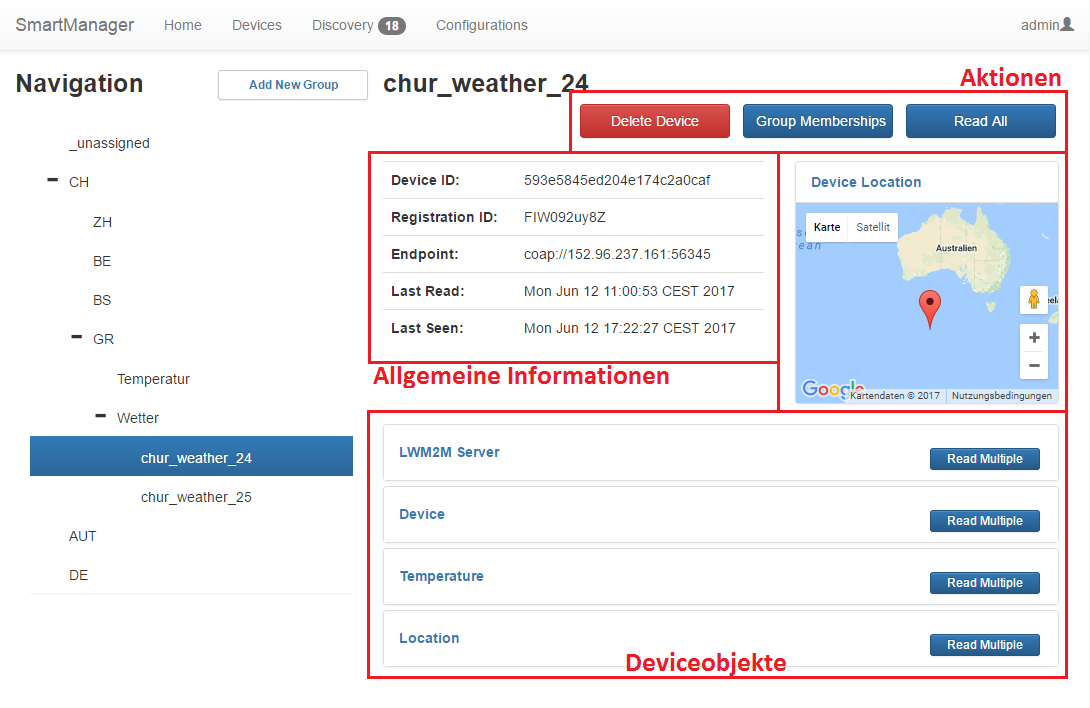
\includegraphics[scale=0.57]{../05_Schlussbericht/images/benutzeranleitung/device_overview.png}
\end{figure} 

Für Devices können Aktionen wie Gruppenmitgliedschaften, Löschen und Lesen ausgeführt werden. Im Bereich der allgemeinen Informationen ist Nützliches auf einen Blick zusammengefasst.
\newpage

\subsubsection{Deviceobjekte}
Im Bereich der Deviceobjekte sind die Deviceattribute verborgen. Klickt man auf ein Objekt, so öffnet sich eine Tabelle mit sämtlichen verfügbaren Ressourcen.
\begin{figure}[H]
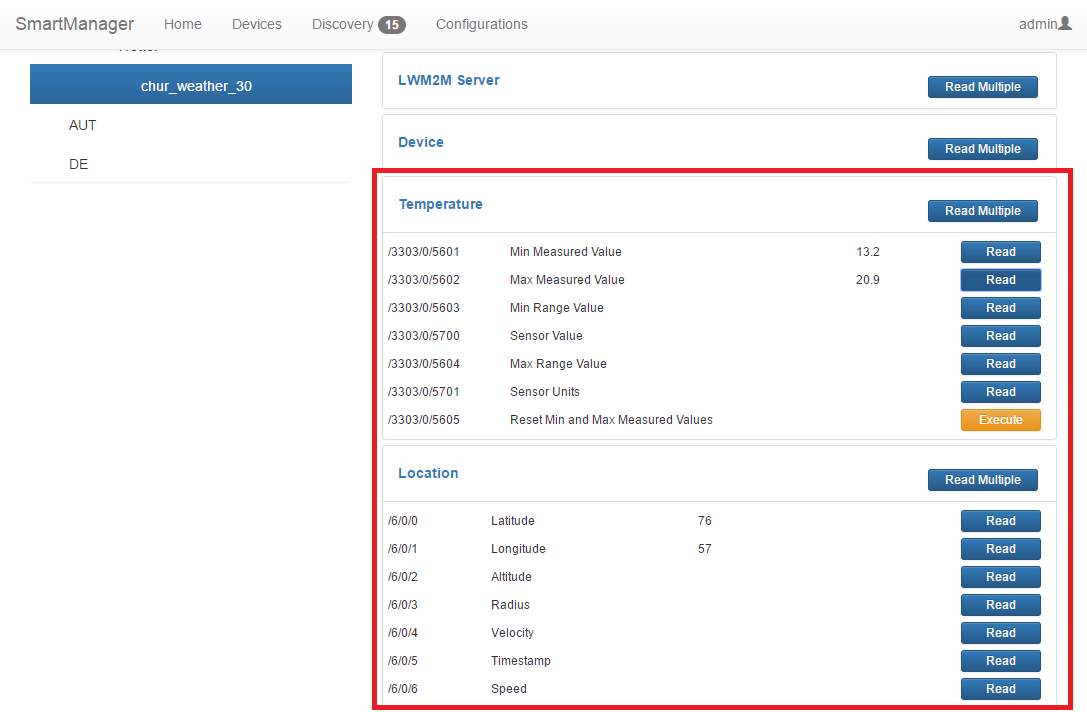
\includegraphics[scale=0.57]{../05_Schlussbericht/images/benutzeranleitung/devicefragment.png}
\end{figure}

Falls man Probleme hat, die einzelnen Zeilen zu interpretieren, sollte die Spezifikation des Ressourcenmodells konsultiert werden. Auf der rechten Seite sind Buttons mit den verfügbaren Aktionen vorhanden.
\newpage

\section{Operationen auf Devices ausführen}
LwM2M unterstützt die vier Operationen ''Read'', ''Write'', ''Execute'' und ''Observe''. Die ''Oberserve''-Funktion ist noch nicht verfügbar. Diese Operationen sind jeweils für eine Ressource definiert und können einzeln ausgeführt werden.

In dieser Applikation ist es ebenfalls möglich, Operationen auf Gruppenebene auszuführen, damit effizient eine grosse Anzahl Devices administriert werden können.

\subsubsection{Execute}
Wählt man in der Gruppenansicht ''Execute'', so kann man für sämtlichen Nachfahren der Gruppe eine Aktion wie Beispielsweise einen Reboot durchführen.

\begin{figure}[H]
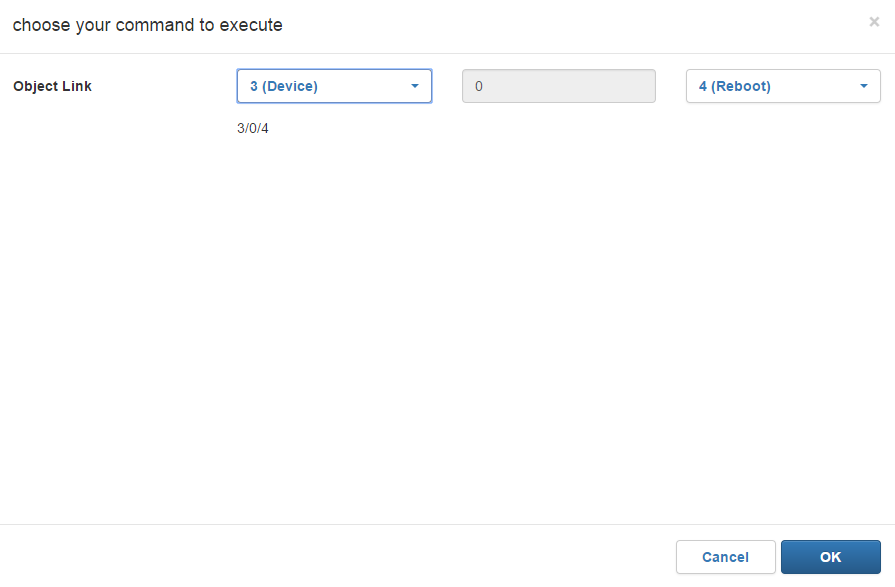
\includegraphics[scale=0.57]{../05_Schlussbericht/images/benutzeranleitung/reboot.png}
\end{figure}

\subsubsection{Write Configuration}
Bestehende Konfigurationen können auf eine ganze Gruppe geschrieben werden. Unter ''Write Configuration'' kann im Drop-Down die gewünschte Konfiguration ausgewählt werden.
\newpage

\subsubsection{Resultate}
Nachdem Schreib- oder Execute-Operationen auf Devices ausgeführt wurden, werden serverseitig Resultate generiert. Somit erhält man einen Überblick über den Erfolg der getätigten Operationen.

\begin{figure}[H]
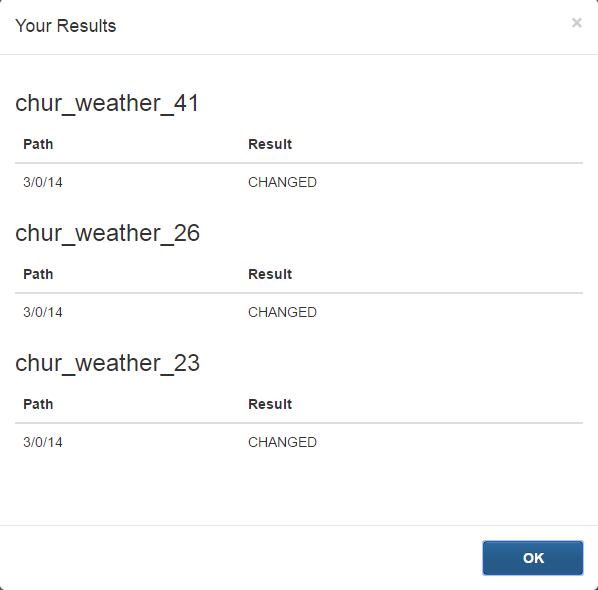
\includegraphics[scale=0.57]{../05_Schlussbericht/images/benutzeranleitung/configresults.png}
\end{figure}
